\section{Locally Linear Embedding (LLE)}

\mode<presentation>{
\begin{frame} 
    \begin{center} \huge
        \secname
    \end{center}
\end{frame}
}

\subsection{Motivation}

\begin{frame}{\subsecname}

Find structure in the data that extends to non-linear manifolds.

\notesonly{

$\textbf{S}$-dataset provides an example of a non-linear manifold.}

\begin{figure}[ht]
	\centering
    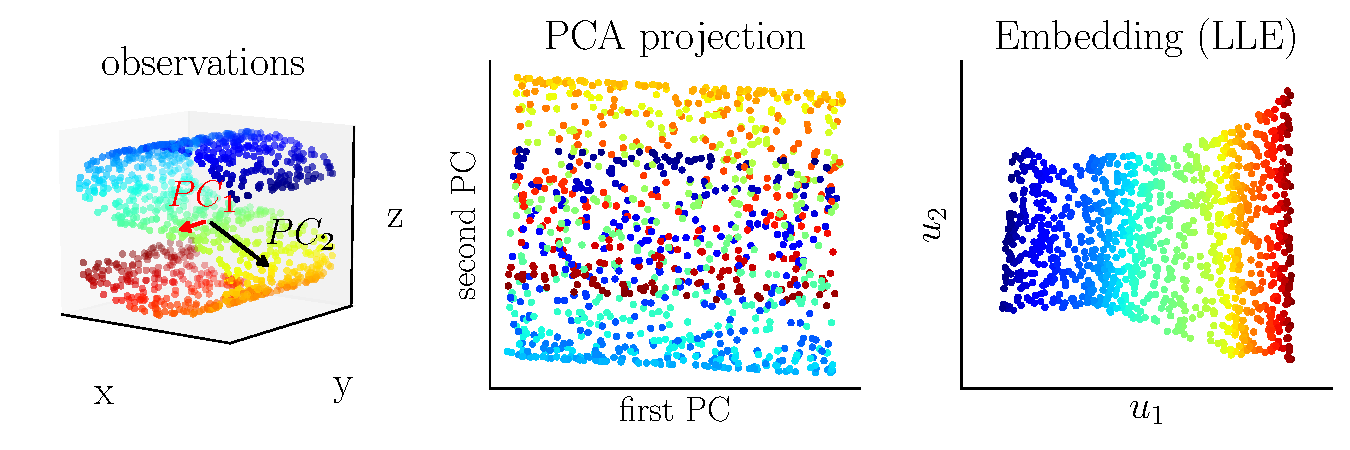
\includegraphics[width=12cm]{img/s_data_proj}
	\notesonly{\caption{The S-dataset, PCA projections and embedding solution. Points are colorized according to their index in the dataset.}}
	\label{fig:s_data_proj_lle}
\end{figure}

\notesonly{
Utilize this to r}\slidesonly{R}educe the dimensionality of the data such that points that lie close \textbf{on} the manifold also lie close in their projection\notesonly{ (we will refer to the projection space which preserving local neighborhoods / ``structure preserving'' as \emph{embedding space})}.

\end{frame}

\notesonly{
Looking at \figref{fig:s_data_proj_lle} we see that the nonlinear manifold is preserved in the LLE embedding, while PCA does not capture the non-linear local structure. The same can be said for \figref{fig:faces_translated_pca_lle}, translating the images from one corner to another has a corresponding translation in the embedded space. In this case we can also infer the coordinates of an image where the face appears in the bottom-left corner in the embedded space.
}

\begin{frame}
\slidesonly{
 \frametitle{Locally Linear Embedding (LLE)}
}
 
\begin{figure}[ht]
	\centering
    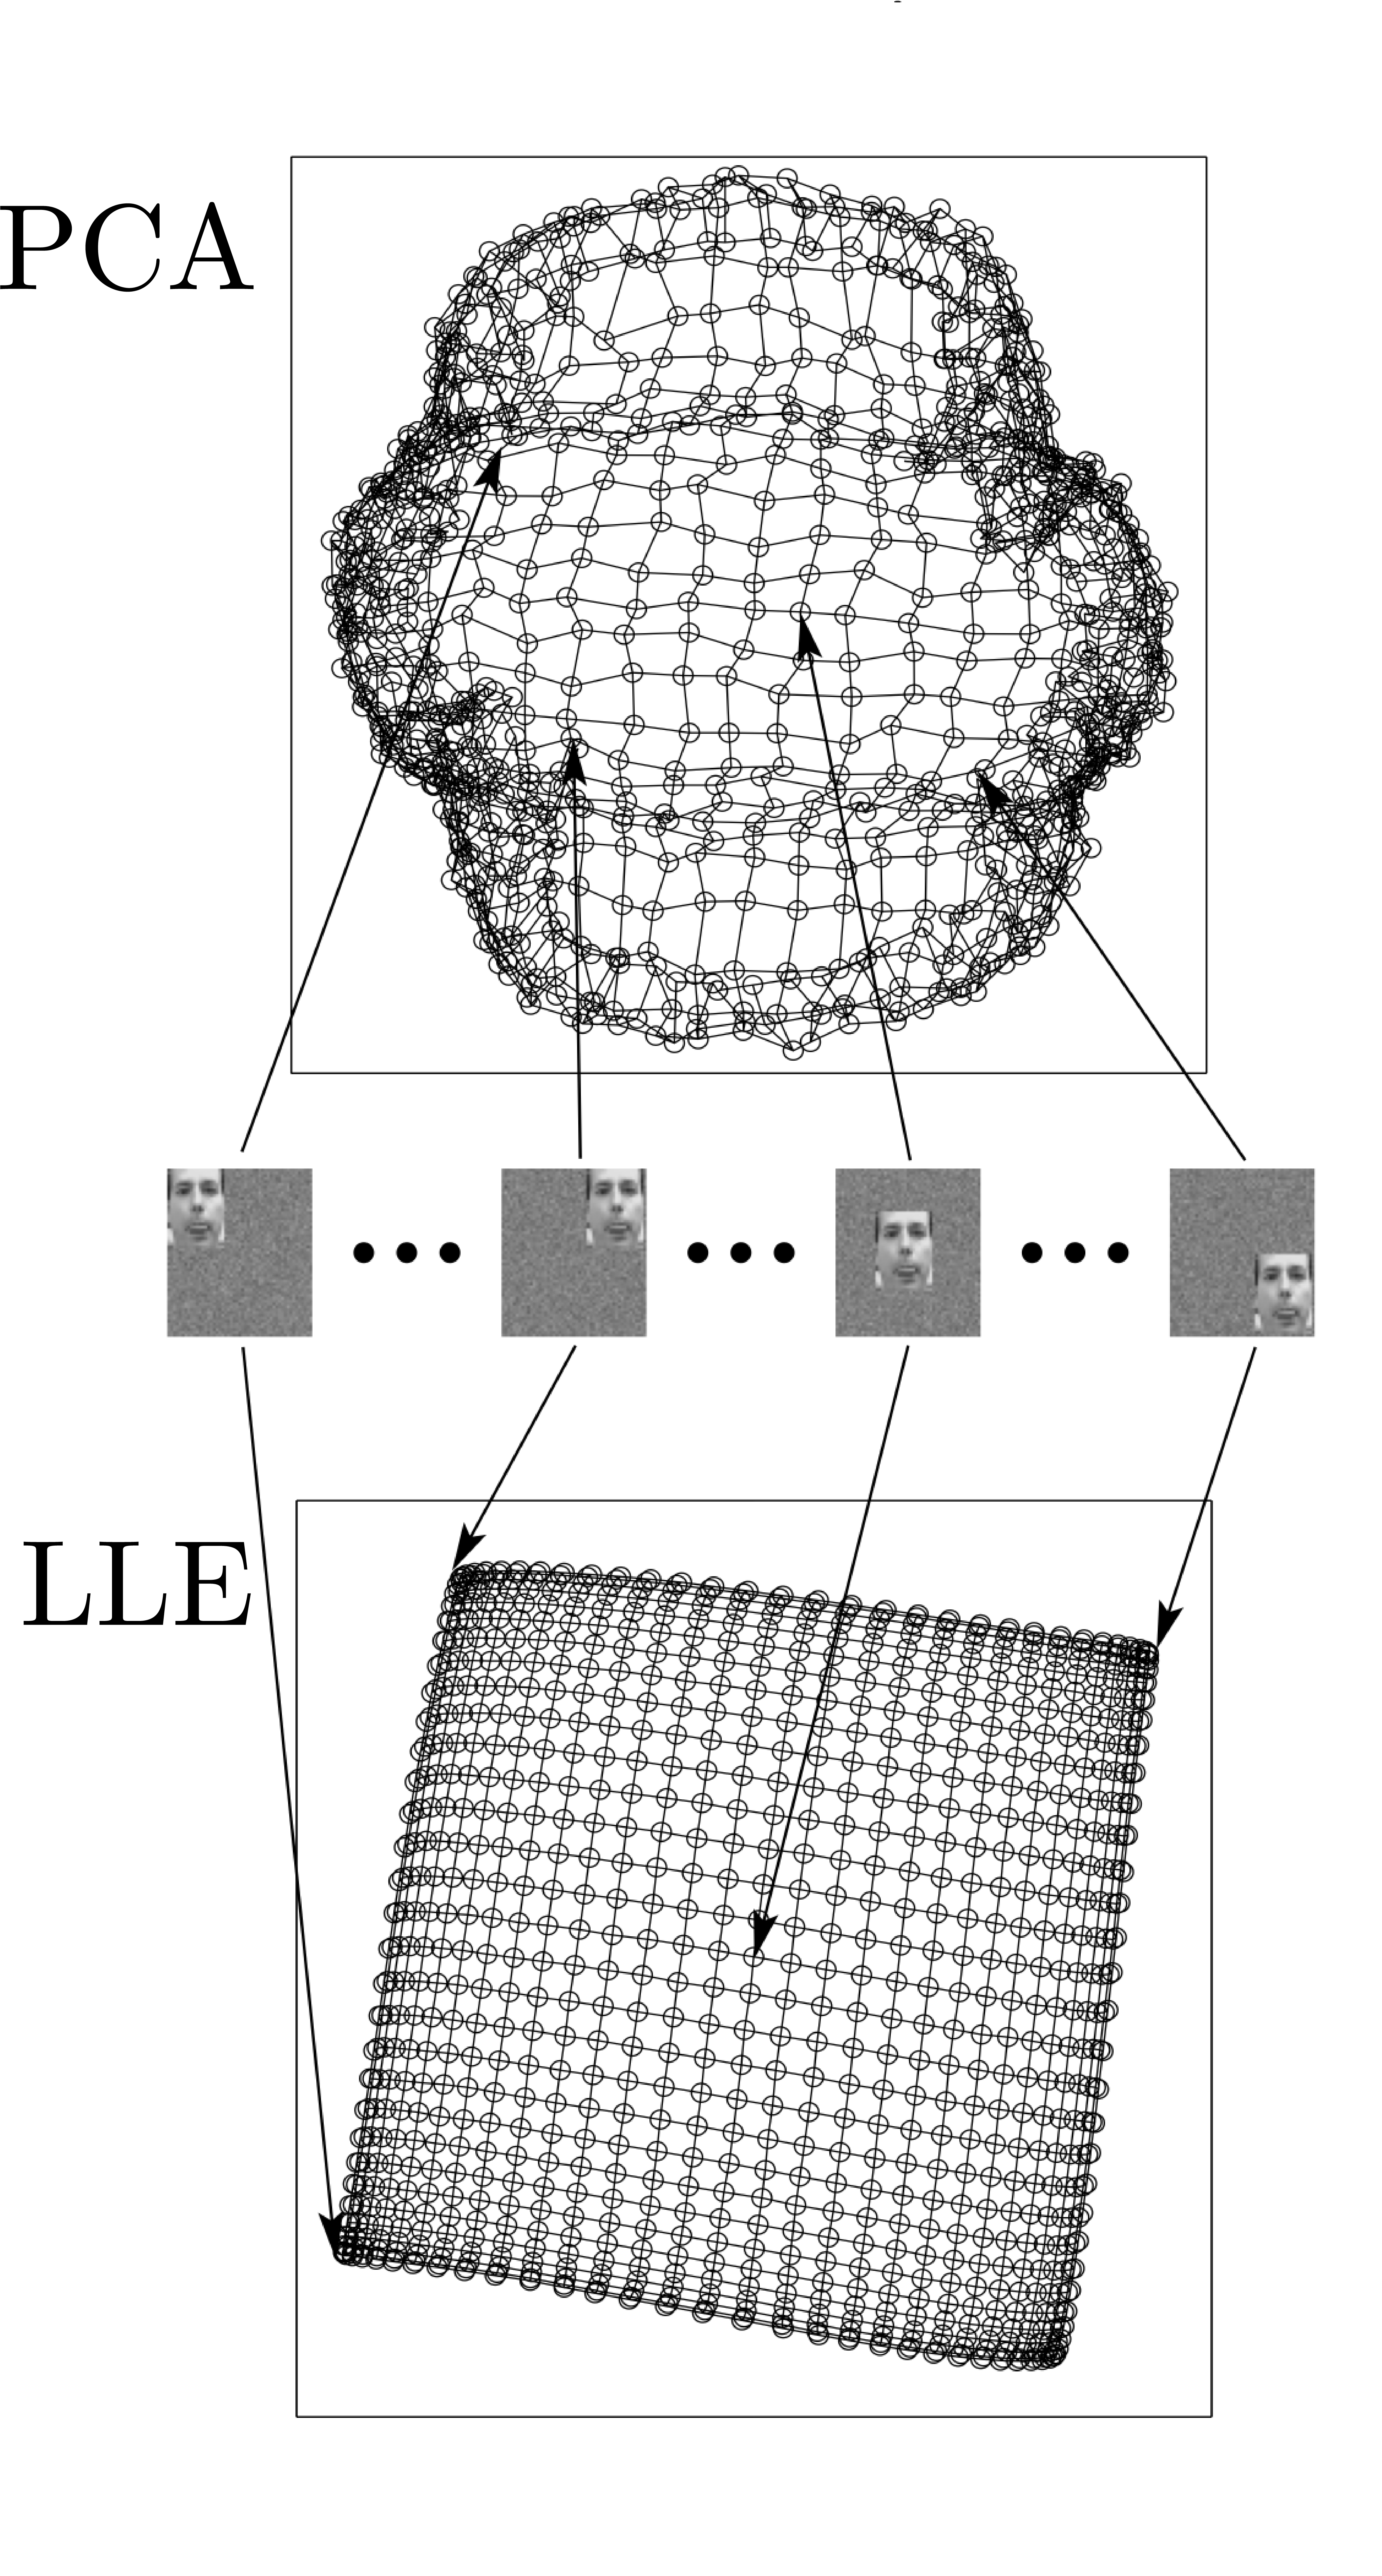
\includegraphics[width=0.3\textwidth]{img/fig3_lle_intro_cropped.png}
	\caption{PCA projections and LLE of translated versions of the same image. What would be the coordinates of the face-in-bottom-left-corner-image be?}
	\label{fig:faces_translated_pca_lle}
\end{figure}
\end{frame}

\subsection{Algorithm outline}

\subsubsection{A representation of local structure}

\begin{frame}{\subsecname:~\subsubsecname}

\notesonly{
LLE is a fairly simple algorithm. }Local structure is preserved by optimizing the projection of a neighborhood of points (PCA finds a projection for all points collectively).

\pause

But first we have to identify the neighborhood.

\end{frame}

\begin{frame}{\subsecname:~\subsubsecname}

\question{How do we ``localize'' the local structure?}

\pause

- through K-nearest neighbors (KNN)

\begin{center}
    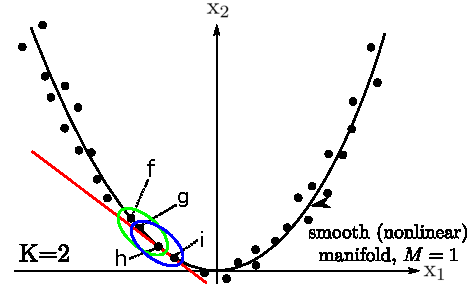
\includegraphics[width=0.6\textwidth]{img/section4_fig11_K2}
    \captionof{figure}{Finding the projection of a neighborhood of points.}
	\label{fig:tangentialk2}
\end{center}

\end{frame}

\begin{frame}{\subsecname:~\subsubsecname}

\slidesonly{
\begin{center}
    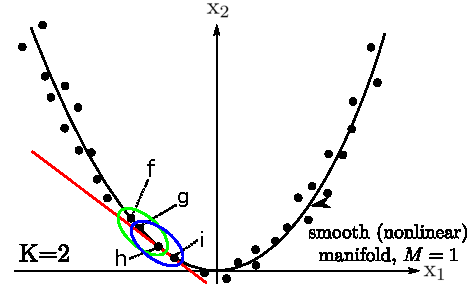
\includegraphics[width=0.5\textwidth]{img/section4_fig11_K2}
    \captionof{figure}{Finding the projection of a neighborhood of points.}
	\label{fig:tangentialk2}
\end{center}
}
\only<1>{
\question{What do we do with the KNN?}
}

\only<2>{
\notesonly{

- We approximate each point as a weighted sum of its KNN.
}
\begin{equation}
\vec{x}^{(\alpha)} \approx \hspace{-3mm} \sum_{\beta \in \operatorname{KNN}(\vec{x}^{(\alpha)})}^{} \hspace{-5mm} \mathrm{W}_{\alpha \beta} \cdot \vec{x}^{(\beta)} \qquad \forall \; \alpha
\end{equation}

The first thing to optimize in LLE are the reconstruction weights $W_{\alpha\beta}$ to yield a good approximation of $\vec x^{(\alpha)}$
}

\end{frame}

\begin{frame}{Optimizing the reconstruction weights}

\begin{align}
\only<1->{
\vec{x}^{(\alpha)} &\approx \hspace{-3mm} \sum_{\beta \in \operatorname{KNN}(\vec{x}^{(\alpha)})}^{} \hspace{-5mm} \mathrm{W}_{\alpha \beta} \cdot \vec{x}^{(\beta)} &\qquad \forall \; \alpha
}
\only<2->{
\intertext{A good approximation is one with minimal squared Euclidean distance:}
\Big\lVert \vec{x}^{(\alpha)} &- \hspace{-3mm} \sum_{\beta \in \operatorname{KNN}(\vec{x}^{(\alpha)})}^{} \hspace{-5mm} \mathrm{W}_{\alpha \beta} \cdot \vec{x}^{(\beta)} \Big\rVert_2^2 \eqexcl \min_{\{W_\alpha\beta\}} &\qquad \forall \; \alpha
}
\end{align}

Next,
\begin{itemize}
\item Formulate a cost function for finding a good approximation for all points $\alpha=1,\ldots,p$ in the dataset,
\item also, store the reconstruction weights into a matrix $\vec W$
\item add constraints
\end{itemize}

\end{frame}

\begin{frame}{Calculate the reconstruction weights}

\begin{align}
E(\vec{W}) =& \sum_{\alpha=1}^{p} \overbrace{\Big\lVert{\vec{x}^{(\alpha)} - \sum_{\beta=1}^{p} \mathrm{W}_{\alpha \beta} \vec{x}^{(\beta)}}\Big\rVert_2^2}^{\substack{\text{reconstruct } \vec{x}^{(\alpha)} \text{ by its } \\ K \text{ nearest neighbors only}}} \;\; \eqexcl \;\; \min_{\vec W}\\
\text{s.t.} \quad &\mathrm{W}_{\alpha \beta} = 0 \text{ if } \beta \notin \operatorname{KNN}(\vec{x}^{(\alpha)}), \\
&\sum_{\beta=1}^{p} \mathrm{W}_{\alpha \beta} = 1 \;\; \text{(The neighborhood has to ``explain'' the point)}
\end{align}



\end{frame}

\begin{frame}{Properties of the reconstruction weights}

\svspace{-5mm}

\slidesonly{
\begingroup
\footnotesize
\begin{align}
E(\vec{W}) =& \sum_{\alpha=1}^{p} \overbrace{\Big\lVert{\vec{x}^{(\alpha)} - \sum_{\beta=1}^{p} \mathrm{W}_{\alpha \beta} \vec{x}^{(\beta)}}\Big\rVert_2^2}^{\substack{\text{reconstruct } \vec{x}^{(\alpha)} \text{ by its } \\ K \text{ nearest neighbors only}}} \;\; \eqexcl \;\; \min_{\vec W}\\
\text{s.t.} \quad &\mathrm{W}_{\alpha \beta} = 0 \text{ if } \beta \notin \operatorname{KNN}(\vec{x}^{(\alpha)}), \\
&\sum_{\beta=1}^{p} \mathrm{W}_{\alpha \beta} = 1 \;\; \text{(The neighborhood has to ``explain'' the point)}
\end{align}
\endgroup
}

\svspace{-15mm}

\begin{minipage}{0.28\textwidth}
\begin{center}
	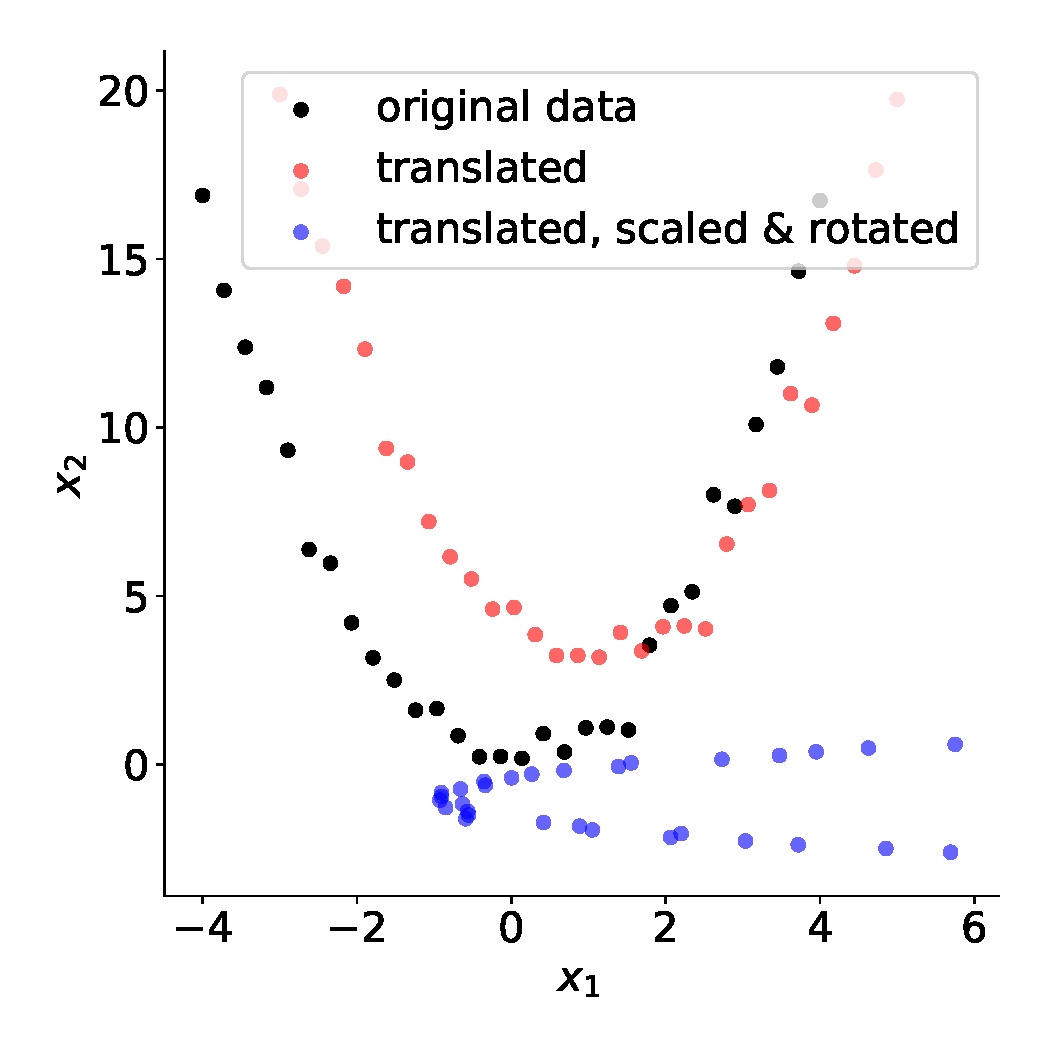
\includegraphics[width=1.2\textwidth]{img/parabola_data}
	\notesonly{\captionof{figure}{2D points describing a parabola.}}
\end{center}
\end{minipage}
\begin{minipage}{0.7\textwidth}
\begin{center}
	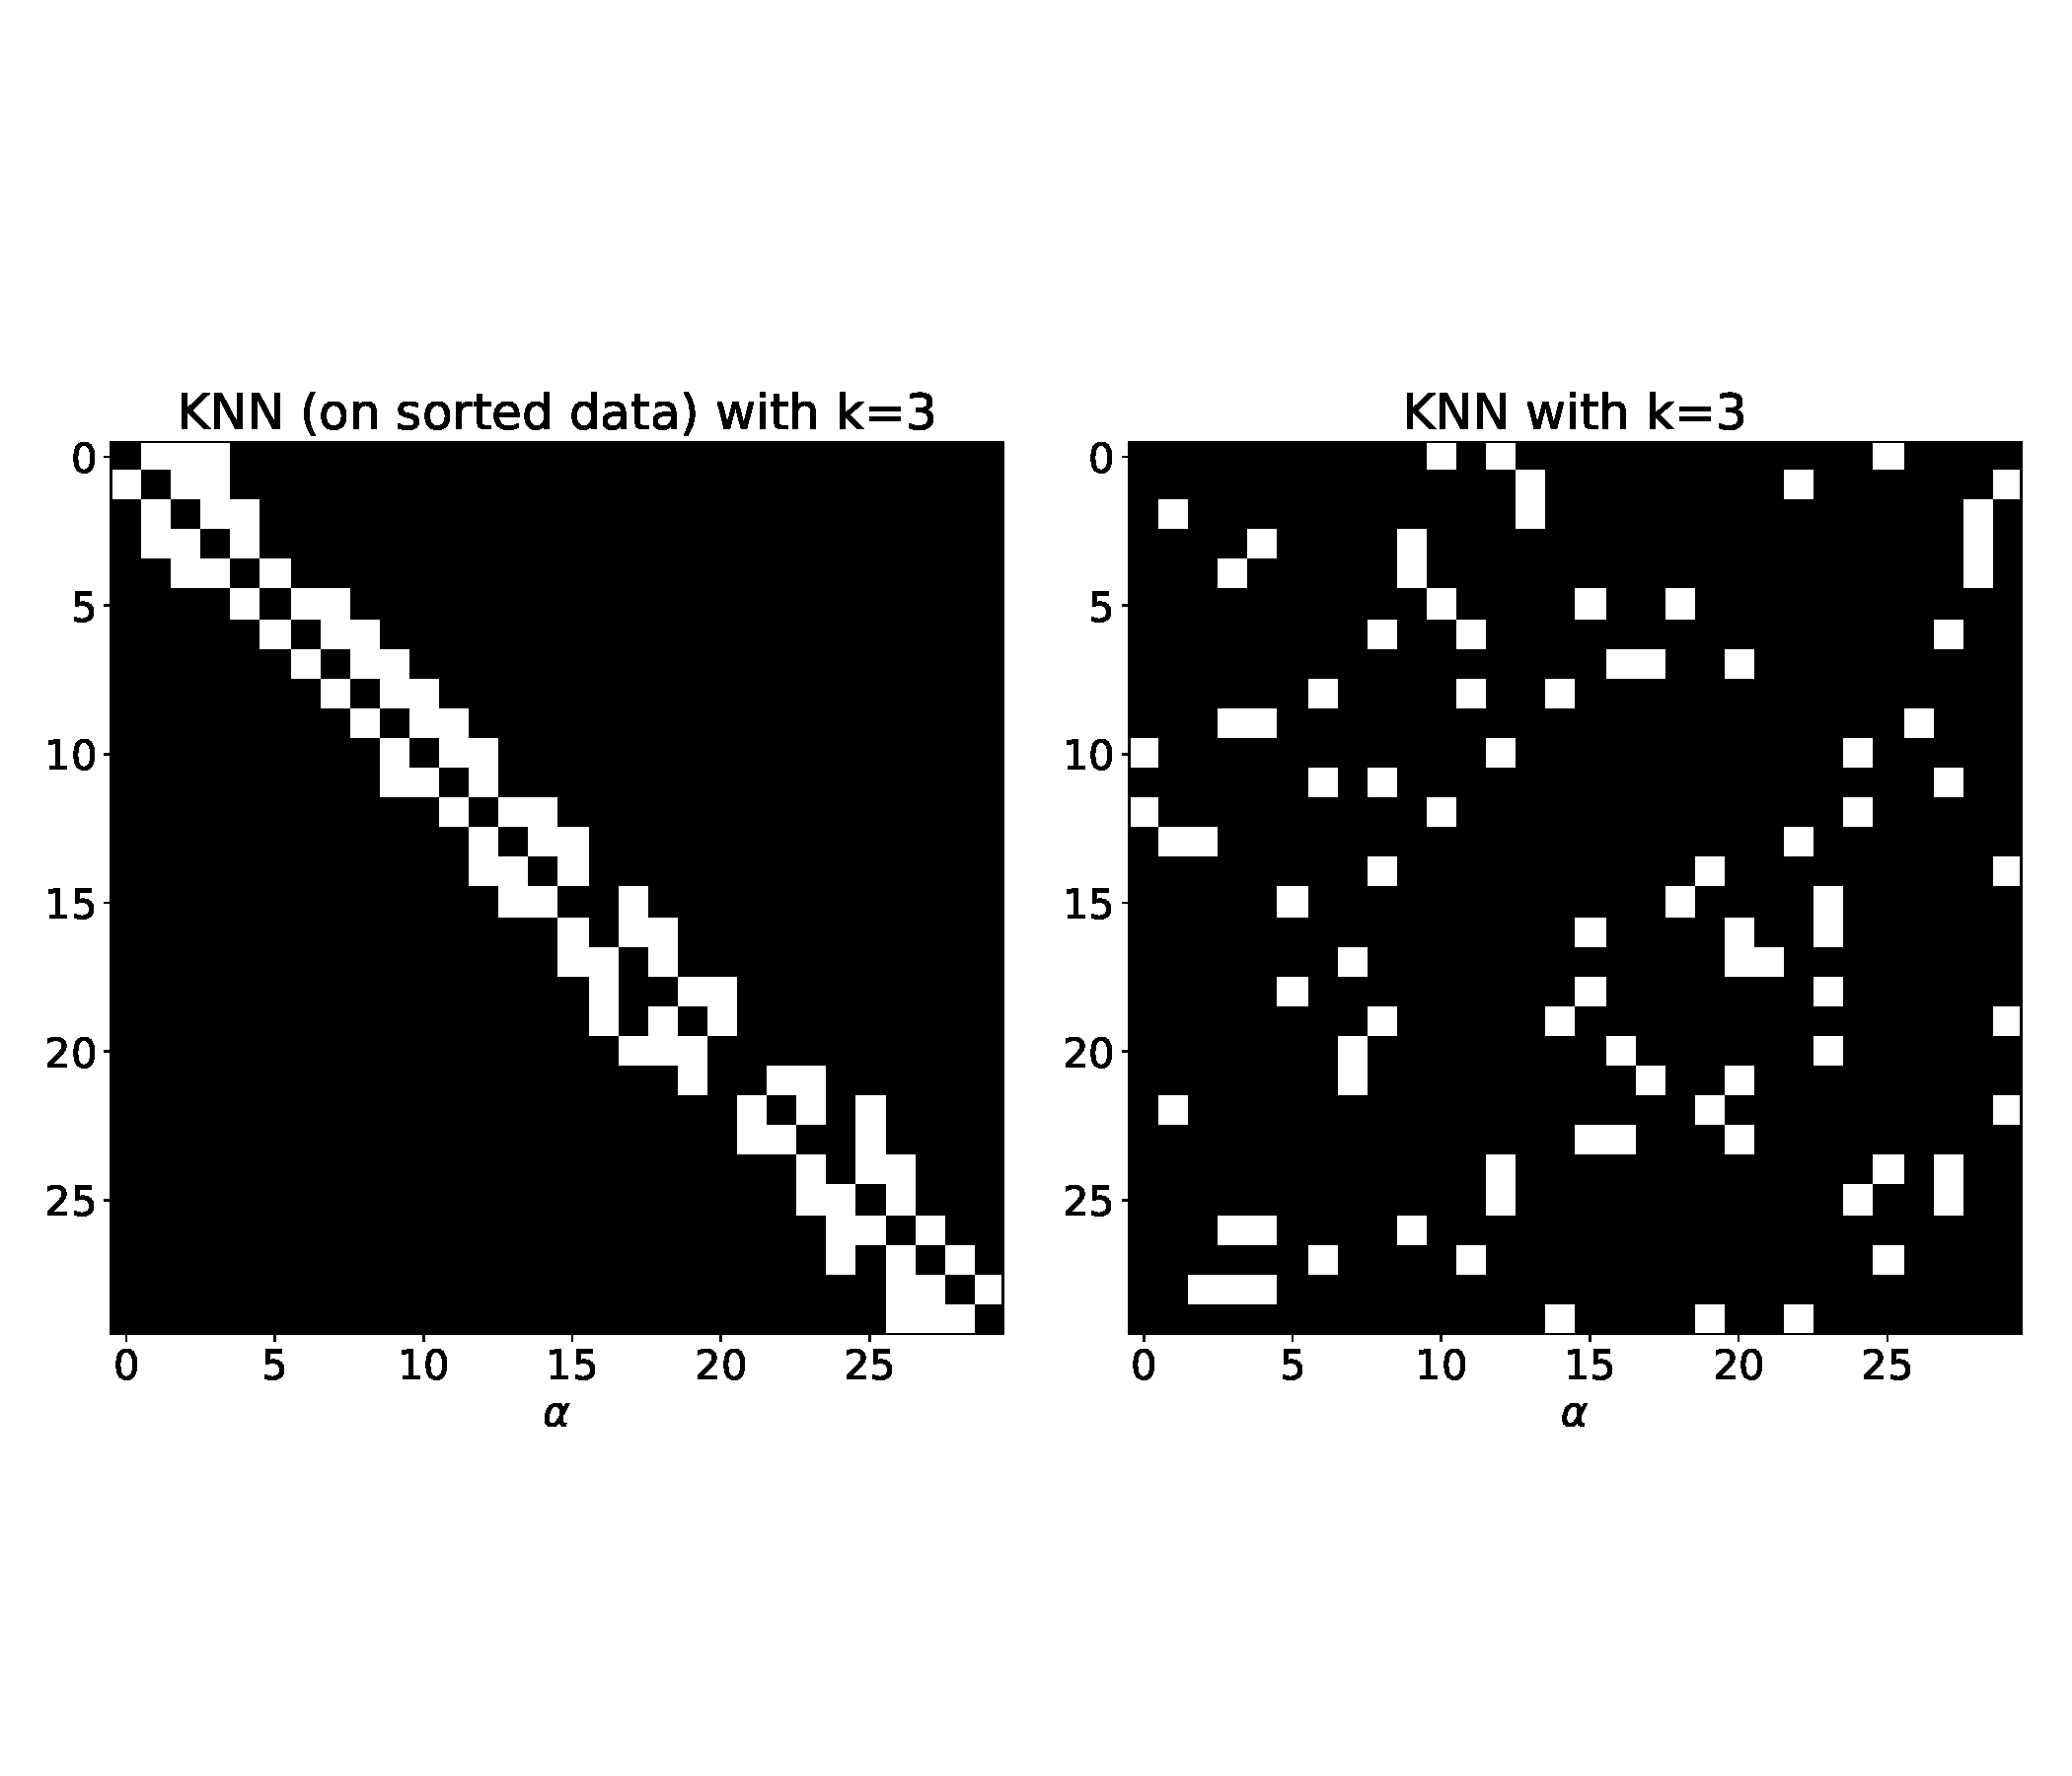
\includegraphics[width=0.95\textwidth]{img/parabola_knn}
	\notesonly{\captionof{figure}{Highlighting the KNN.}}
\end{center}
\end{minipage}

\end{frame}

\subsubsection{The embedding coordinates}

\begin{frame}{\subsubsecname}

Local structure is now stored in the reconstruction weights $\vec W$.

We have used $\vec W$ to reconstruct any point $\vec x^{(\alpha)}$ in the input space $\R^N$.

The embedding space has to preserve the local structure.

If the embedding space maps every point $\vec x^{(\alpha)}$ to an $M$-dimensional space with 
coordinates $\vec u^{(\alpha)} \in \R^M$, then the following aproximation:

\begin{equation}\vec{u}^{(\alpha)} \approx \hspace{-3mm} \sum_{\beta \in \operatorname{KNN}(\vec{x}^{(\alpha)})}^{} \hspace{-3mm} \mathrm{W}_{\alpha \beta} \cdot \vec{u}^{(\beta)}
\end{equation}

should hold as well.

\end{frame}

\begin{frame}{Finding the embedding coordinates}

The reconstruction weights in $\vec W$ remain \emph{fixed}.

The embedding coorindates are found by minimizing the approximation error of every point $\vec u^{(\alpha)}$ through its local neighborhood:

\begin{equation}
	F(\vec U) =
    \sum_{\alpha=1}^{p} 
	\bigg(  \vec{u}^{(\alpha)}  - \sum_{\beta=1}^{p} W_{\alpha \beta} \vec{u}^{(\beta)}
	\bigg) ^ 2
\end{equation}

where $\vec U \in \R^{M,p}$ is the embedded dataset with all $p$ points.

\end{frame}

\begin{frame}
The binomial expansion leads to an equivalent formulation of the cost function as:

\svspace{-5mm}

\begin{align}
F(\vec{U}) =& 
\sum_{\alpha, \beta=1}^{p}
\Big\lbrack
\delta_{\alpha \beta} - \mathrm{W}_{\alpha \beta} - \mathrm{W}_{\beta \alpha} + \sum_{\gamma=1}^{p} \mathrm{W}_{\gamma \alpha} \mathrm{W}_{\gamma \beta} \Big\rbrack (\vec{u}^{(\alpha)})^\top \vec{u}^{(\beta)} \\
=& \sum_{\alpha, \beta=1}^{p} g_{\alpha \beta} (\vec{u}^{(\alpha)})^\top \vec{u}^{(\beta)}
\end{align}

\question{What do we expect for the embedding coordinates?}

\pause

\svspace{-3mm
}
\begin{itemize}
\item[-] Tranlsation, scaling and rotaiton of the original dataset $\vec X$ should yield the same embedding coordinates $\vec U$.
\item[-] The above invariances are already properties of the reconstruction weights $\vec W$.
\item[-] Minimizing the squared Euclidean distance enables the above invariances.
\item[-] We still have to prevent the trivial solution of $\vec u^{(\alpha)} = \vec 0 \;\; \forall \;\; \alpha$
\end{itemize}

\end{frame}

\begin{frame}{A constrained optimization problem}

minimize $F(\vec{U}) = \sum_{\alpha, \beta=1}^{p} g_{\alpha \beta} (\vec{u}^{(\alpha)})^\top \vec{u}^{(\beta)}$
\begin{align}
\quad \text{s.t.} \quad
%&\sum_{\alpha=1}^{p} \vec{u}^{(\alpha)} = 0,\quad \text{(remove translation freedom)} \\
&\frac{1}{p} \sum_{\alpha=1}^{p} \vec{u}^{(\alpha)} (\vec{u}^{(\alpha)})^\top = \vec{I} \quad \text{(prevent trivial solution } \vec{u}^{(\alpha)} = \vec{0})
\end{align}

\end{frame}

\begin{frame}

Reformulating $F(\vec U)$ may provide intuition to finding the embedding coordinates $\vec U$:

\begingroup
\small
\begin{align}
\intertext{with $\sum_{\alpha, \beta=1}^{p} g_{\alpha \beta} u_i^{(\alpha)} u_i^{(\beta)}$}
F(\vec U) =& \sum_{i=1}^M \sum_{\alpha, \beta=1}^{p} g_{\alpha \beta} u_i^{(\alpha)} u_i^{(\beta)}
\intertext{and having all $\{g_\alpha\beta\}$ stored in a matrix $\vec G = \Big( \vec{I} - \vec{W}^\top \Big) \Big( \vec{I} - \vec{W} \Big)$ we can rewrite $F(\vec U)$ as}
=& \sum_{i=1}^M  \vec u_{(i)}^\top \vec G \, \vec u_{(i)} = 
\sum_{i=1}^M \vec u_{(i)}^\top \vec u_{(i)} \lambda_{i}
\end{align}
\endgroup

\end{frame}

\begin{frame}

\slidesonly{
\begin{equation}
F(\vec U)
= \sum_{i=1}^M  \vec u_{(i)}^\top \vec G \, \vec u_{(i)} = 
\sum_{i=1}^M \vec u_{(i)}^\top \vec u_{(i)} \lambda_{i}
\end{equation}

Recall from PCA:
\begin{equation}
	\underbrace{ \vec{e}_a^\top \vec{C} \, \vec{e}_a }_{
		\text{objective} }
	- \lambda \underbrace{ \big( \vec{e}_a^\top\vec{e}_a - 1 \big) }_{
			\text{constraints} }
	\eqexcl \max
\end{equation}
}

Finding $\vec U$ involves finding the eigenfunctions of $\vec G$.

\begin{equation}
\vec G \vec e_j = \lambda_j \vec e_j
\end{equation}

\question{Which eigenvectors do we look for?}

\notesonly{
-Unlike PCA, which tries to maximize the Lagrangian, we're trying to minimize $F(\vec U)$.
Therefore, we will be looking for the eigenvectors with \emph{smallest} eigenvalues.

Local structure is described by the eigenvectors with small eigenvalues.

In order to obtain $M$ embedding coordinates, we find the $M+1$ eigenvectors with smalles eigenvalues and discard the last eigenvector. In this case the last eigenvector will always be associated with a $\lambda$ of zero, so there's no information about the manifold there.
}
\end{frame}

\mode<article>{
%\begin{frame}%[label=g_alpha_beta_proof]{Supplementary Material}
%\begin{textblock}{5}(13,0.075)
	%\hyperlink{g_alpha_beta_slide}{\beamerbutton{back to lecture}}
%\end{textblock}
	Derivation of $g_{\alpha \beta}$ in the cost function
	$F(\vec U) =
    \sum_{\alpha=1}^{p} 
	\bigg(  \vec{u}^{(\alpha)}  - \sum_{\beta=1}^{p} W_{\alpha \beta} \vec{u}^{(\beta)}
	\bigg) ^ 2
    $ 
    for finding the optimal embedding coordinates.\\
    First, a brief refresher on binomial expansion of vectors:
	%{\footnotesize{}
    \begin{align}
    \big( 
		\vec{a}
		- \vec{b}
	\big) ^ 2 
    &= \big(  \vec{a} - {\color{blue}\vec{b}} \big)^\top \big(  \vec{a} - {\color{red}\vec{b}} \big)\\
    &= \vec a^\top \vec a 
    - \vec a^\top {\color{red}\vec{b}}
    - {\color{blue}\vec{b}^\top} \vec a 
    - {\color{blue}\vec{b}^\top} {\color{red}\vec{b}}
    \end{align}\\
    
    Let $\;\vec a = \vec u^{(\alpha)}\;$ and 
    $\;{\color{red}
    \vec{b}=\sum_{\beta=1}^{p} W_{\alpha \beta} \vec{u}^{(\beta)}
    } \Leftrightarrow {\color{blue}
    \vec{b}^{\top}=\sum_{\beta=1}^{p} 
    W_{\beta \alpha} \left(\vec{u}^{(\beta)}\right)^\top
    }
    $
    
    \question{Why do we flip the indices from 
    ${\color{red} W_{\alpha \beta}}$ to ${\color{blue} W_{\beta \alpha}}$?}\\
    The reason we flip the Transposing $\vec u^{(\beta)}$ 
    
    \begin{align}
	= &\sum_{\alpha=1}^{p} 
	\bigg[ 
	(\vec{u}^{(\alpha)})^2
	- 2 \sum_{\beta=1}^{p} W_{\alpha \beta} (\vec{u}^{(\alpha)} )^\top \vec{u}^{(\beta)}
	+
	\sum_{\beta=1, \gamma=1}^{p} W_{\alpha \beta} W_{\alpha \gamma} (\vec{u}^{(\beta)} )^\top \vec{u}^{(\gamma)}
	\bigg]
	\\
	= &\sum_{\alpha=1}^{p} 
	\bigg[ 
	(\vec{u}^{(\alpha)})^2
	- \sum_{\beta=1}^{p} W_{\alpha \beta} (\vec{u}^{(\alpha)} )^\top \vec{u}^{(\beta)}
	- \sum_{\beta=1}^{p} W_{\beta \alpha} (\vec{u}^{(\beta)} )^\top \vec{u}^{(\alpha)}
	\\~~~~~~~&+
	\sum_{\beta=1}^{p} 
		\sum_{\gamma=1}^{p} 
		\bigg(
			W_{\gamma \alpha} 
			W_{ \gamma \beta}
		\bigg) 
		(\vec{u}^{(\alpha)} )^\top \vec{u}^{(\beta)}
	\bigg]
	\\
	= &\sum_{\alpha, \beta=1}^{p} 
	\bigg\{ \underbrace{
		\delta_{\alpha \beta}
		- W_{\alpha \beta}
		- W_{\beta \alpha}
		+
		\sum_{\gamma=1}^{p} 
			W_{\gamma \alpha} W_{\gamma \beta} }_{=g_{\alpha \beta}}
	\bigg\}
	(\vec{u}^{(\alpha)} )^\top \vec{u}^{(\beta)}
	\end{align}
    %}
%\end{frame}
}

\subsection{Remarks}

\begin{frame}{Remarks}


\begin{minipage}{0.47\textwidth}
\begin{center}
	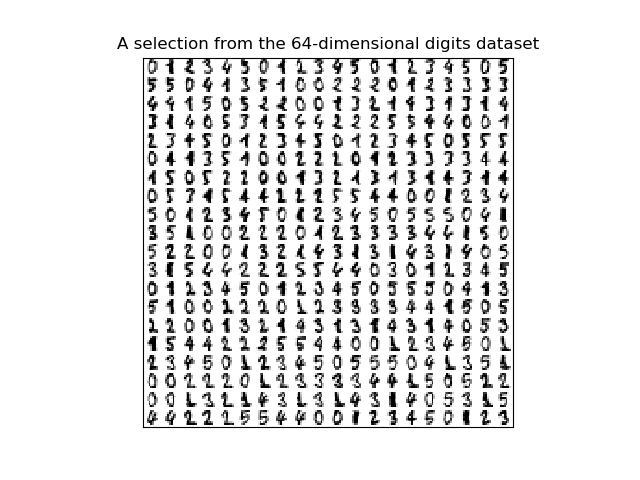
\includegraphics[width=0.9\textwidth]{img/digits}
	\notesonly{\captionof{figure}{Digits data.}}
\end{center}
\end{minipage}
\begin{minipage}{0.47\textwidth}
\begin{center}
	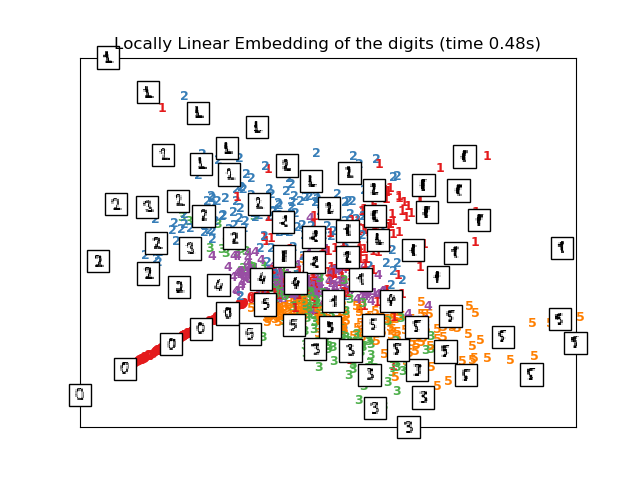
\includegraphics[width=0.95\textwidth]{img/digits_lle}
	\notesonly{\captionof{figure}{2D Embedding of the digits data using LLE.}}
\end{center}
\end{minipage}

\pause

\begin{minipage}{0.47\textwidth}
\begin{center}
	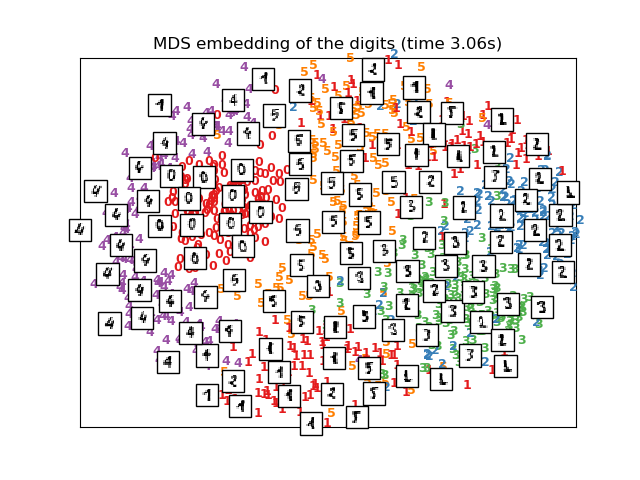
\includegraphics[width=0.9\textwidth]{img/digits_mds}
	\notesonly{\captionof{figure}{2D Embedding of the digits data using multi-dimensional scaling ``pairwise PCA''.}}
\end{center}
\end{minipage}
\begin{minipage}{0.47\textwidth}
\begin{center}
	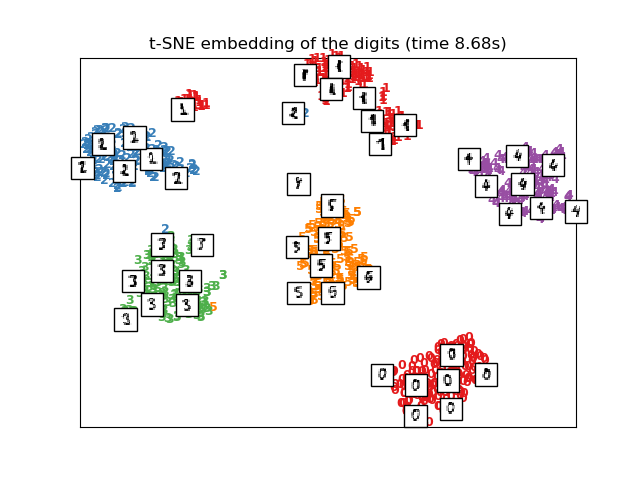
\includegraphics[width=0.95\textwidth]{img/digits_tsne}
	\notesonly{\captionof{figure}{2D Embedding of the digits data using t-SNE.}}
\end{center}
\end{minipage}

\notesonly{
Embedding figures for digits data were obtained from \href{https://scikit-learn.org/stable/auto_examples/manifold/plot_lle_digits.html}{here}
}
\end{frame}
